{\let\clearpage\relax \chapter{绘图}}

\section{函数图}
\subsection{二维函数图}
绘制函数$f(x)=sin(x)$和$g(x)=cos(x)$在定义域$[-2\pi,2\pi]$上的图像。对于函数$f(x)=sin(x)$,我们使用red和\verb|/tikz/line width={1pt}|来使其更显眼。\LaTeX 默认取点少,我们使用samples=x来控制取点数,使函数图像更为平滑。


\begin{latex}{}
\addplot[domain=-2*pi:2*pi,samples=200,red,/tikz/line width={1pt}]{sin(deg(x))};
\addplot[domain=-2*pi:2*pi]{cos(deg(x))};
\end{latex}

\begin{center}
	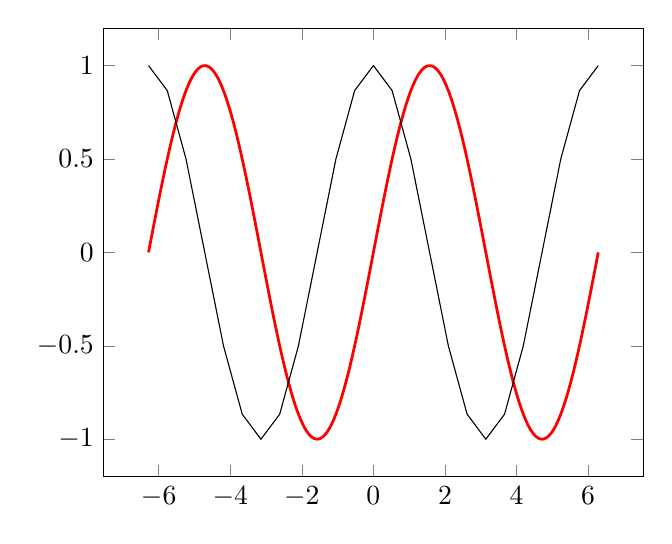
\begin{tikzpicture}
	\begin{axis}
	\addplot[domain=-2*pi:2*pi,samples=200,red,/tikz/line width={1pt}]{sin(deg(x))};
	\addplot[domain=-2*pi:2*pi]{cos(deg(x))};
	\end{axis}
	\end{tikzpicture}
\end{center}

绘图命令里面是可以直接输入函数表达式的,使用如下命令可以直接绘制函数$x^2$在定义域$[-10:10]$上的图像。

\begin{latex}{}
\addplot[domain=-10:10,red,samples=50]{x^2}
\end{latex}

\begin{center}
	\begin{tikzpicture}
	\begin{axis}[
		xlabel={$x$},
		ylabel={$y$},
		]
	\addplot[domain=-10:10,red,samples=50]{x^2};
	\legend{$x^{2}$}
	\end{axis}
\end{tikzpicture}
\end{center}

\subsection{三维函数图}
绘制函数$f(x,y)=x^2+y^2$的三维函数图像。
其中参数\qd{colorbar}可以为函数图添加一个彩色条。


\begin{latex}{}
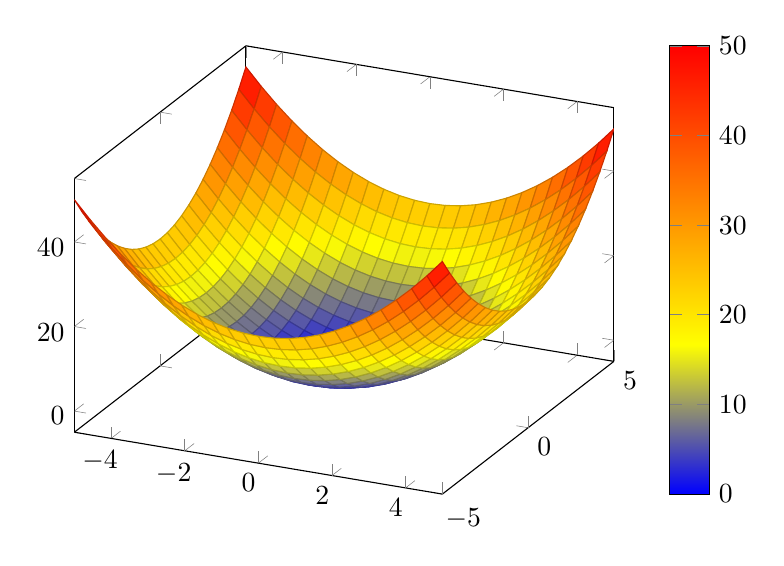
\begin{tikzpicture}
\begin{axis}[colorbar]
\addplot3[surf]{x^2+y^2};
\end{axis}
\end{tikzpicture}
\end{latex}


\begin{center}
	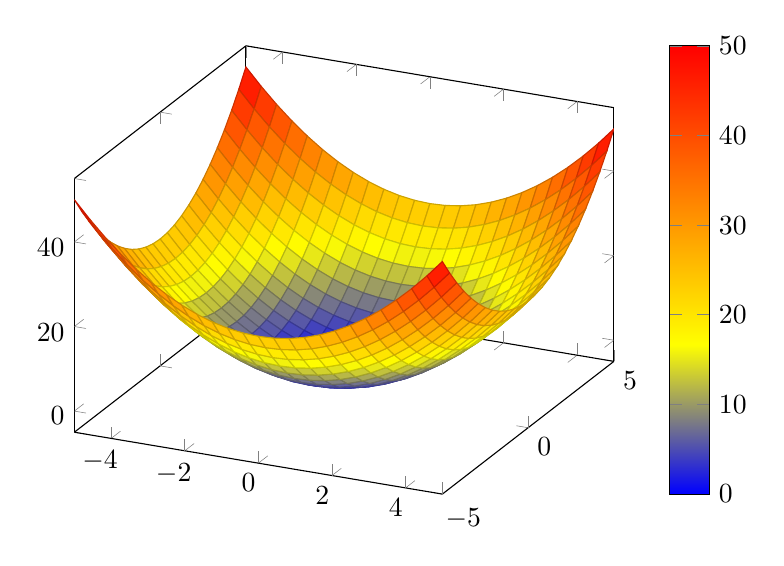
\begin{tikzpicture}
		\begin{axis}[colorbar]
		\addplot3[surf]{x^2+y^2};
		\end{axis}
	\end{tikzpicture}
\end{center}

绘制函数$g(x,y)=\dfrac{sin(\sqrt{x^2+y^2})}{\sqrt{x^2+y^2}}$的三维函数图像。


\begin{latex}{}
\addplot3[surf,samples=50,domain=-10:10]{sin(deg(sqrt(x^2+y^2)))/sqrt(x^2+y^2)};
\end{latex}


\begin{center}
	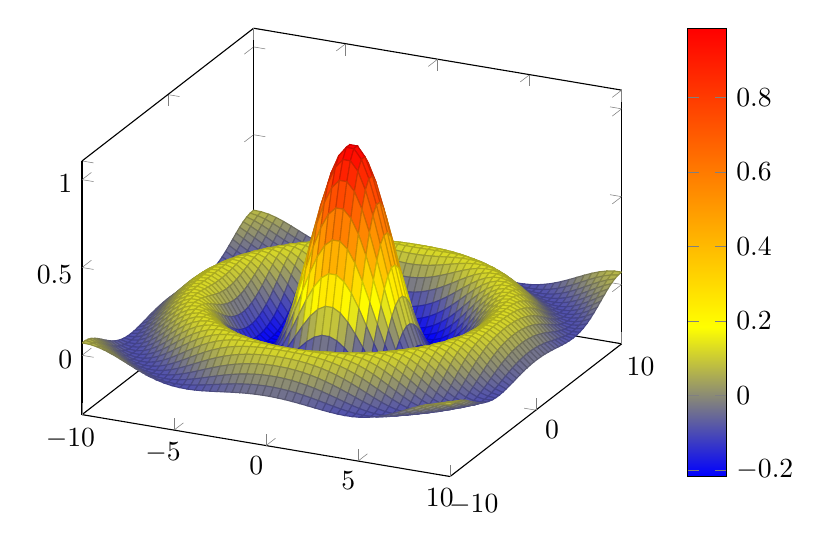
\begin{tikzpicture}
	\begin{axis}[
		colorbar,
%		hide axis,
%		colormap/cool,
]
	\addplot3[surf,samples=50,domain=-10:10]{sin(deg(sqrt(x^2+y^2)))/sqrt(x^2+y^2)};%可用surf,mesh
%	\addlegendentry{$\frac{sin(r)}{r}$}         %添加图例
%	\legend{$\frac{sin(r)}{r}$}
	\end{axis}
	\end{tikzpicture}
\end{center}

\subsection{隐函数图像}

\section{线图}
对于折线图而言,使用sharp plot可以得到折线图,而使用smooth可以得到平滑曲线图。这些命令在addplot的设置里面添加。一些其他基础设置如下所示。

\begin{latex}{}
\item grid=major		%显示网格线
\item mark=x			%设置数据点标记类型
\end{latex}


\section{条形图}

\section{从外部数据作图}

从外部文件加载数据,例如从COMSOL导出数据为txt文档,在\LaTeX 中可以直接读取其中的数据作图,只要指定正确的数据路径即可。

\begin{latex}{}
\addplot[blue,smooth,domain=0:1,/tikz/line width={0.4pt}] table[x=x,y=y] {body/data.txt};
\end{latex}


\begin{center}
	\begin{tikzpicture}
	\begin{axis}[
		title=线图$u+log(x)/(2\pi)$,
		xlabel={弧长},
		ylabel={$u+log(x)/(2\pi)$},
		width=12cm,
		]
	\addplot[blue,smooth,domain=0:1,/tikz/line width={0.4pt}] table[x=x,y=y] {body/data.txt};
	\legend{小小的图例测试}
	\end{axis}
\end{tikzpicture}
\end{center}


